\chapter[Conclusão]{Conclusão}

Esta pesquisa buscou analisar o contexto de SLAM dentro dos limites da Robótica Educacional, com o objetivo de estudar a
viabilidade da utilização de técnicas renomadas na comunidade de robótica para solucionar o problema de SLAM. De acordo com o apresentado ao
longo da pesquisa, a comunidade de robótica busca solucionar o problema de SLAM utilizando diversas
técnicas e estratégias. Entretanto, boa parte da comunidade concorda com a utilização de algumas estratégias, como o processamento remoto,
apresentado na tabela \ref{tab:resultadosRevisao}. Visto isso, este trabalho buscou seguir as estratégias mais utilizadas e reconhecidas
 para o contexto da pesquisa, como a utilização da arquitetura de processamento remoto e a utilização do Filtro de Partículas.

Como o contexto alvo da pesquisa faz referência a Robótica Educacional, buscou-se utilizar ferramentas simples,
presentes no kit de robótica Mindstorm NXT e disponíveis em ambientes educacionais, advindos de baixo investimento. Foi possível
estudar, analisar e adaptar estratégias e técnicas de auto-localização no contexto limitado da Robótica Educacional. Esta análise mostrou
que a utilização de técnicas como o Filtro de Partículas se torna viável quando os estudantes possuem liberdade para alterar o robô e o
ambiente, trabalhando de maneira empírica para minimizar a margem de erro presente na solução.

De acordo com \cite{teachingWithRoboticKit}, a solução de problemas a partir do estudo empírico (pesquisa empírica) é uma característica
importante no contexto da Robótica Educacional. Esta característica favorece o trabalho em equipe e a solução de problemas de forma autodidata,
incendivando o interesse e a dedicação dos alunos participantes, ainda de acordo com \cite{teachingWithRoboticKit}. Desse modo, a questão
da necessidade de adaptação do robô e ambiente, que poderia ser considerada prejudicial em diversos contextos, se torna uma característica
importante e positiva no contexto da Robótica Educacional.

Esta pesquisa obteve importantes resultados, tanto em relação a revisão sistemática sobre o tema pesquisado, quanto em relação
a implementação da solução, identificando fontes críticas de erro, maneiras de minimizar estas fontes e a viabilidade da aplicação
no contexto educacional. Para que a pesquisa se complete, deve-se analisar, ainda, a integração da auto-localização e do mapeamento
de ambientes, ambos implementados, completamente e parcialmente, durante esta pesquisa. Desse modo, deve-se destacar as lacunas
deixadas pela pesquisa, apresentando os trabalhos futuros para que novos interessados possam seguir e completar o estudo sobre o SLAM
no contexto educacional.

Os trabalhos futuros desta pesquisa são:

\begin{itemize}
  \item Refinar implementação do mapeamento de ambientes:

    Para que esta implementação possa ser integrada com facilidade no módulo de auto-localização, a mesma deve gerar um mapa
    no formato \textit{svg}, destacando as paredes presentes no ambiente em forma de linhas. De acordo com as características
    apresentadas na seção \ref{sec:fontes_de_erros}, é possível adiantar que a solução do mapeamento de ambientes deve incluir uma
    camada de filtragem do resultado, que busca linearizar a representação das paredes e obstáculos.

    Esta linearização é necessária devido, principalmente, a característica do sensor de distância utilizado (sonar). A Figura \ref{img:mapeamento_result}
    apresenta o resultado obtido sem a utilização de um filtro para linearizar a saída obtida. Para que o mapeamento de ambientes seja
    incluído na solução geral, este deve, primeiramente, minimizar a margem de erro e incorporar uma camada de filtro para linearizar
    o resultado do mapeamento.

    {\centering
    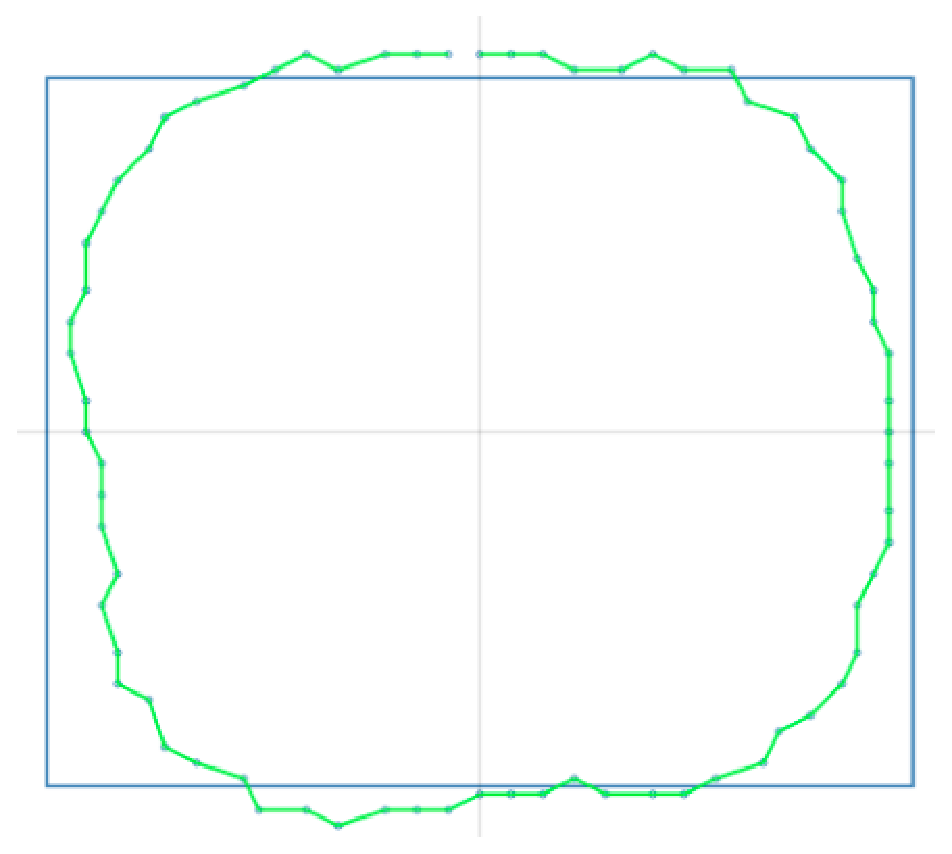
\includegraphics[scale=0.7]{figuras/mapeamento_result.eps}
    \captionof{figure}{Mapeamento de Ambientes - Implementação Inicial.}
    \label{img:mapeamento_result}
    \par}

  \item Refinar solução do sequestro do robô:

    A solução do sequestro do robô, um dos motivos favoráveis a escolha do Filtro de Partículas para implementação desta solução,
    se encontra, no fim desta pesquisa, implementada e funcional. Entretanto, a solução utilizada durante a pesquisa envolve, apenas,
    a solução de um "sequestro" durante a etapa dos ciclos de filtragem, onde o robô navega pelo ambiente buscando se encontrar no mesmo.

    Como trabalho futuro, pode-se incluir a ideia de solucionar o problema do sequestro do robô a qualquer momento. Ou seja, após os ciclos
    de filtragem, quando o robô já conhece sua localização atual, pode ocorrer um "sequestro do robô". Neste caso, o robô deve perceber
    as mudanças no ambiente, chegando a conclusão de que o mesmo não se encontra mais no local conhecido. Ao concluir que o robô não se
    encontra na posição conhecida, o mesmo deve iniciar novamente o processo de auto-localização, criando o conjunto de partículas e
    executando os ciclos de filtragem. Esta solução não precisa seguir a estratégia, para execução dos ciclos de filtragem, adotada durante esta pesquisa,
    já que esta estratégia envolve a iteração do pesquisador/usuário durante a execução dos ciclos. Esta execução, no caso do "sequestro do robô",
    pode ser automatizada, prosseguindo sem a necessidade da participação do usuário.

  \item Integrar mapeamento e auto-localização, completando o SLAM:

    Durante esta pesquisa foi implementada a solução da auto-localização utilizando o Filtro de Partículas. Além disso, foi iniciada
    a implementação da solução para mapeamento de ambientes, durante a prova de conceito desta pesquisa. Como trabalho futuro,
    deve-se integrar estas duas soluções, possibilitando  a auto-localização e o mapeamento de ambientes simultâneo (SLAM).

    A API utilizada para solucionar o problema de SLAM exige a utilização de um mapa pronto no formato "svg", para que as partículas
    sejam distribuídas no mesmo. Entretando, sabe-se que, durante as primeiras fases do SLAM, o mapa se encontra parcialmente concluído,
    o que inviabilizaria a utilização da API leJOS, neste caso. Porém, a partir da experiência obtida durante a pesquisa, observou-se
    uma estratégia viável para integração destes dois módulos. Nesta estratégia, o robô constrói o mapa com as informações que possui
    e preenche o restante com informações fictícias, possibilitando o "fechamento" do mapa e, com isso, a utilização do mesmo
    no algoritmo do Filtro de Partículas.

\end{itemize}
